\chapter{Исследования характеристик источника тока}

\section{Цель работы}

Исследовать зависимость полной мощности, полезной мощности, мощности потерь, падения напряжения во внешней цепи и КПД источника от силы тока в цепи.

\section{Ход работы}

\subsection{График зависимости напряжения U от силы тока I}

\begin{table}[h]
	\caption{}
	\begin{tabularx}{\textwidth}{|c|X|X|X|X|X|X|X|X|X|X|X|X|X|X|X|}
		\hline
		R, Ом & 100 & 200 & 300 & 400 & 500 & 600 & 700 & 800 & 900 & 1000 \\ \hline
		U, В & $1.0$ & $2.5$ & $3.6$ & $4.7$ & $5.5$ & $6.1$ & $7.1$ & $8.0$ & $8.5$ & $9.1$ \\ \hline
		I, А & $0.019$ & $0.017$ & $0.015$ & $0.014$ & $0.013$ & $0.012$ & $0.010$ & $0.009$ & $0.008$ & $0.007$ \\ \hline
	\end{tabularx}
\end{table}

\begin{figure}[h]
	\centering
	\caption{График зависимости напряжения $U$ от силы тока $I$}
	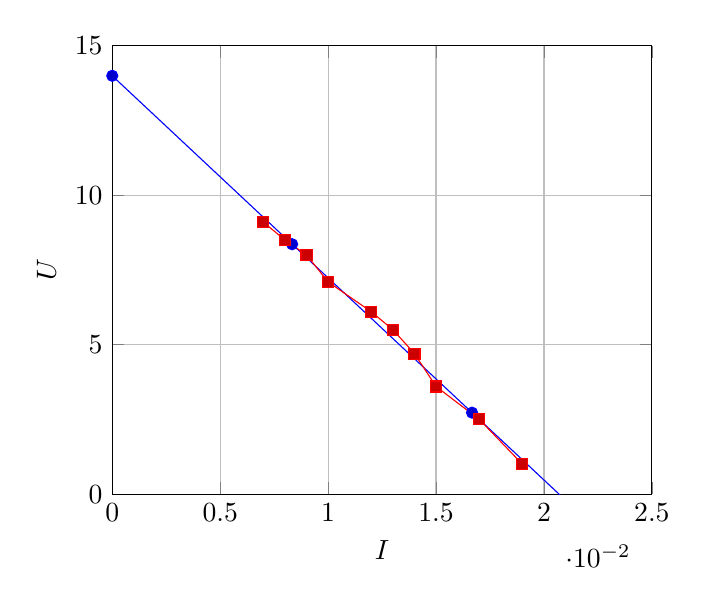
\begin{tikzpicture}
	\begin{axis}[
		domain=0:0.2,
		xlabel=$I$,
		ylabel=$U$,
		xmin=0, xmax= 0.025,
		ymin=0, ymax=15,
		grid=major
		]
	\addplot {13.995 - 676.211*x};
	\addplot coordinates {
		(0.019, 1.0)
		(0.017, 2.5)
		(0.015, 3.6)
		(0.014, 4.7)
		(0.013, 5.5)
		(0.012, 6.1)
		(0.010, 7.1)
		(0.009, 8.0)
		(0.008, 8.5)
		(0.007, 9.1)
	};
	\end{axis}
	\end{tikzpicture}
\end{figure}

Экстраполируя график до пересечения с осями координат, получаем:
\[
\varepsilon = 13.995 \text{ [В]}, I_K = 0.0206 \text{ [А]}
\]

Определим внутреннее сопротивление источника $r$
\[
I = \frac{U}{R+r} \Leftrightarrow r = \frac{U-R \cdot I}{I} \Leftrightarrow r= \frac{U}{I} - R
\]

\begin{table}[h]
	\caption{}
	\begin{tabularx}{\textwidth}{|c|X|X|X|X|X|X|X|X|X|X|X|X|X|X|X|}
		\hline
		R, Ом & 100 & 200 & 300 & 400 & 500 & 600 & 700 & 800 & 900 & 1000 \\ \hline
		U, В & $1.0$ & $2.5$ & $3.6$ & $4.7$ & $5.5$ & $6.1$ & $7.1$ & $8.0$ & $8.5$ & $9.1$ \\ \hline
		I, А & $0.019$ & $0.017$ & $0.015$ & $0.014$ & $0.013$ & $0.012$ & $0.010$ & $0.009$ & $0.008$ & $0.007$ \\ \hline
		r, Ом & $-47.3$ & $-52.9$ & $-60$ & $-64.2$ & $-76.9$ & $-91.6$ & $10$ & $88.9$ & $162.5$ & $300$ \\ \hline
	\end{tabularx}
\end{table}

\[
r = \frac{\varepsilon}{I_K} = \frac{13.995}{0.0206} = 679.3689320388 \text{ [Ом]}
\]

Рассчитаем мощности $P$, $P_1$, $P_2$ и КПД $\eta$ для измеренных значений силы тока. Построим график зависимостей этих величин от силы тока.

\[
P = P_1+ P_2, P_1 = \varepsilon \cdot I  - I^2\cdot r, P_2 = I^2 \cdot r
\]

\begin{figure}[h]
	\centering
	\caption{График зависимости мощностей от силы тока $I$}
	\begin{tikzpicture}
	\begin{axis}[
	domain=0:0.2,
	xlabel=$I$,
	ylabel=$P$,
	xmin=0, xmax= 0.025,
	ymin=0, ymax=0.3,
	grid=major
	]
	\addplot {13.995 * x - x * x * 679};
	\addplot {x * x * 679};
	\addplot {13.995 * x};	
	\end{axis}
	\end{tikzpicture}
\end{figure}